\chapter{Introduction}\label{ch:intro}

%%% Big Data intro

In recent years there has been a concerted effort to apply computer vision techniques to challenging problems which can have a positive societal impact. A highly important area where computer vision can help is conservation \cite{weinstein_computer_2018}. One of the main goals of conservation research is to monitor animal populations in their distribution area, undertaking abundance estimates to inform policy change. This is most commonly performed using capture-recapture surveys where researchers identify the presence of individuals and estimate abundance of animals in an area to produce population estimates \cite{constantine_abundance_2012, bigg_assessment_1982, sharpe_indian_2019, van_bressem_visual_2018, arso_civil_changing_2019, cheney_long-term_2014}. These surveys can be classified as invasive where animals are physically trapped, tagged, and released \cite{norris_tagging_1970, hobbs_bowhead_1982, andrews_best_2019}, or non-invasive where monitoring is performed passively such as via the collection of vast numbers of images. 

Photo-id is one of the main non-invasive capture-recapture methods utilised by cetacean researchers \cite{hammond_individual_1990, evans_monitoring_2004}. Surveys are usually undertaken from vessels at sea, although monitoring from coastlines or aircraft may also be utilised \cite{payne_long_1986, forney_seasonal_1998, wursig_methods_1990}. The methodology is employed for the monitoring of multiple cetacean species, with proven use cases in a range of studies \cite{sharpe_indian_2019, miragliuolo_rissos_2004, feyrer_origin_2021, bigg_assessment_1982}. Outside of cetaceans, photo-id has further found use studying other marine life \cite{holmberg_estimating_2009, reisser_photographic_2008} and terrestrial species \cite{goswami_application_2007, clapham_automated_2020}.

All capture-recapture methodologies rely on the target species having some form of individually identifiable markings. Depending on the species, different parts of the body are the primary identifying feature; for dolphins this is usually the dorsal fin as this body part is most likely to be visible above the waterline \cite{sharpe_indian_2019, baird_population_2009}. During photo-id surveys, researchers often focus on long lasting stable markers such as dorsal fin shape, notches, scarring, and pigmentation \cite{wursig_photographic_1977, lockyer_observations_1990, mann_cetacean_2000}. These markings can be difficult to capture in detail due to the free roaming nature of the animals causing high variances in angles of approach, direction of travel, distance from camera, and surfacing elevation. This is exacerbated when dealing with cetacean species which travel in pods, making it difficult to distinguish the individuals present.

Marine photo-id can be extremely labour and cost intensive compared to on-land surveys, which rely on the use of camera traps placed in stationary locations to capture images when they detect movement. This setup is not possible at sea due to a lack of stationary objects to attach devices to and rapid movement in the observed scene due to waves causing the camera to trigger -- producing a high false positive rate. 

Upon survey completion, photo-id data must be analysed and individuals identified to produce a catalogue. Images collected during surveys are large in size and contain significant amounts of background noise. Historically curation of this data has been a manual process that often takes longer than the entire data collection period \cite{tyson_moore_rise_2022}, further increasing labour and costs. For example, previous efforts to create an individual photo-id catalogue from surveys undertaken by Newcastle University's School of Natural \& Environmental Science's Marine MEGAfauna Lab took around three months. As such, any techniques to speed up the cataloguing process would be welcomed both by researchers and their funding bodies, affording more time to work on the application of data, for example to inform mitigation and policy change, rather than curation. 

\begin{figure}
	\begin{center}
		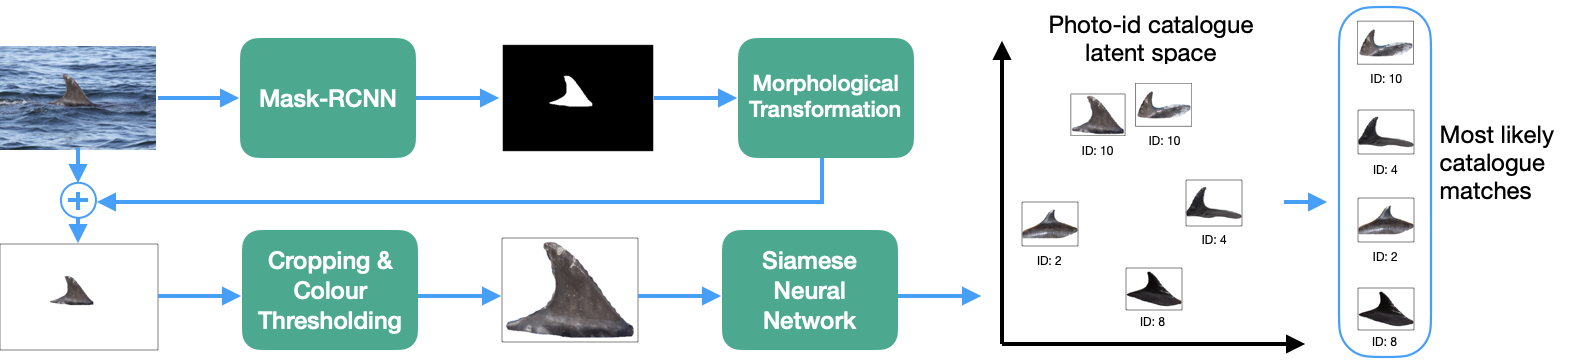
\includegraphics[width=\linewidth]{Chapter1/figs/pipeline_compact.png}
	\end{center}
	\caption{A high level overview of data flow through the proposed system.}
	\label{fig:pipeline}
\end{figure}

This thesis details a system for fully automatic catalogue matching based on unprocessed photo-id imagery. This is achieved through a pipeline of trained computer vision models and robust post-processing techniques capable of automatic fin detection and most likely catalogue matching based on latent space similarity, a visualisation of which can be seen in Figure \ref{fig:pipeline}. As photo-id surveys are not guaranteed to capture all individuals in a given geographic area, naive approaches such as training a simple image classifier on existing catalogue examples would not suffice as they are incapable of flagging previously uncatalogued individuals. Images are passed through a Mask R-CNN \cite{he_mask_2017} dorsal fin detector, removing the need for manual data pre-processing. Detections are then post-processed ready for fine-grain, few-shot catalogue matching utilising a Siamese Neural Network trained using triplet loss \cite{schroff_facenet_2015} and online semi-hard triplet mining to create a latent space based on the provided catalogue. Matches are obtained using the Euclidean distances between an input and class prototypes stored in the latent space, allowing for the flagging of potentially uncatalogued individuals to the researcher

\section{Research Aim \& Contributions}\label{ch:intro,sec:AimsAndContributions}

The high level aim of this thesis is to:

\begin{flushleft}
	\textbf{Design, implement, and evaluate a system for fully automatic catalogue matching based on unprocessed photo-id fieldwork imagery.}
	\bigbreak\noindent Implicit in this aim are a number of research questions:
\end{flushleft}

\begin{enumerate}
	\item Is coarse-grain detection of cetaceans in large-scale, noisy, above water photo-id imagery possible with high levels of accuracy? 
	\item Can detections be automatically post-processed in such a way as to both reject likely false positives and remove noise, whilst retaining identifiable markings?
	\item ls it possible to perform highly accurate most likely photo-id catalogue matching based on extreme fine-grain information, even when operating on few-shot data?
	\item How generalisable are the above concepts to changes in species of interest and spatio-temporal shifts?
\end{enumerate}

%TODO: Contributions, where they are in the thesis

\section{Thesis Structure}\label{ch:intro,sec:Structure}

%TODO: Structure of thesis

\section{Related Publications}\label{ch:intro,relatedPublications}

%TODO: Publications


%%%%%%%%%%%%%%%%%%%%%%%%%%%%%%%%%%
% All nomenclature here for ease
\nomenclature[z-CNN]{CNN}{Convolutional Neural Networks}
\nomenclature[z-CV]{CV}{Computer Vision}
\nomenclature[z-CPU]{CPU}{Central Processing Unit}
\nomenclature[z-GPU]{GPU}{Graphical Processing Unit}
\nomenclature[z-SGD]{SGD}{Stochastic Gradient Descent}
\nomenclature[z-SGDR]{SGDR}{Stochastic Gradient Descent with Restarts}
\nomenclature[z-ReLU]{ReLU}{Rectified Linear Unit}
\nomenclature[z-FCN]{FCN}{Fully Convolutional Network}
\nomenclature[z-RPN]{RPN}{Region Proposal Network}
\nomenclature[z-VM]{VM}{Virtual Machine}
\nomenclature[z-MCZ]{MCZ}{Marine Conservation Zone}
\nomenclature[z-RIB]{RIB}{Rigid Inflatable Boat}
\nomenclature[z-NDD20]{NDD20}{Northumberland Dolphin Dataset 2020}
\nomenclature[z-SMRU]{SMRU}{Sea Mammal Research Unit}
\nomenclature[z-PCA]{PCA}{Principle Component Analysis}
\nomenclature[z-SURF]{SURF}{Speeded-Up Robust Features}
\nomenclature[z-SIFT]{SIFT}{Speeded-Up Robust Features}
\nomenclature[z-TPE]{TPE}{Tree-structured Parzen Estimator}
\nomenclature[z-KNN]{KNN}{K-Nearest Neighbours}
\nomenclature[z-SDRP]{SDRP}{Sarasota Dolphin Research Program}
